\chapter{Introduction}

This paper is the result of the seminar on "Advanced Database Systems" at the University of Applied Science Rapperswil. The paper shall cover all the necessary concepts of "Streaming Database Systems" and investigating one particular product for its abilities. The product is determined to be "Apache Spark Streaming" which is well known to be used in companies handling big data flows for daily business like Uber\cite{uber}, Netflix and Pinterest.

\section{Motivation}
Modern \Gls{RDBMS} show the perfect snapshot of the past, while modern businesses rely heavily on data, these concepts become limiting. While there is a need for storage and persistence, where \Gls{RDBMS}s are still in their prime, there is another need for real time data processing. Real time data processing can be useful to give an accurate anticipation about the future. This use case is a driving force to justify an new database concept for data streams - the \Gls{DSMS} is born. 
\\
\subsection{Fundamentals of \Gls{RDBMS}}
To gain further insights and justify the need for new concepts, it is necessary to have at the look at already given and proven concepts. Fundamentals of database systems require to understand the concept of the CAP-Theorem. The CAP-Theorem was first introduced by Eric Brewer in 2000 and later verified.
\\
\blockquote{When designing distributed web services, there are three properties that are commonly desired: consistency, availability, and partition tolerance. It is impossible to achieve all three.} \cite[S. 1]{Gilbert:2002:BCF:564585.564601}

\begin{figure}[H]
	\centering
	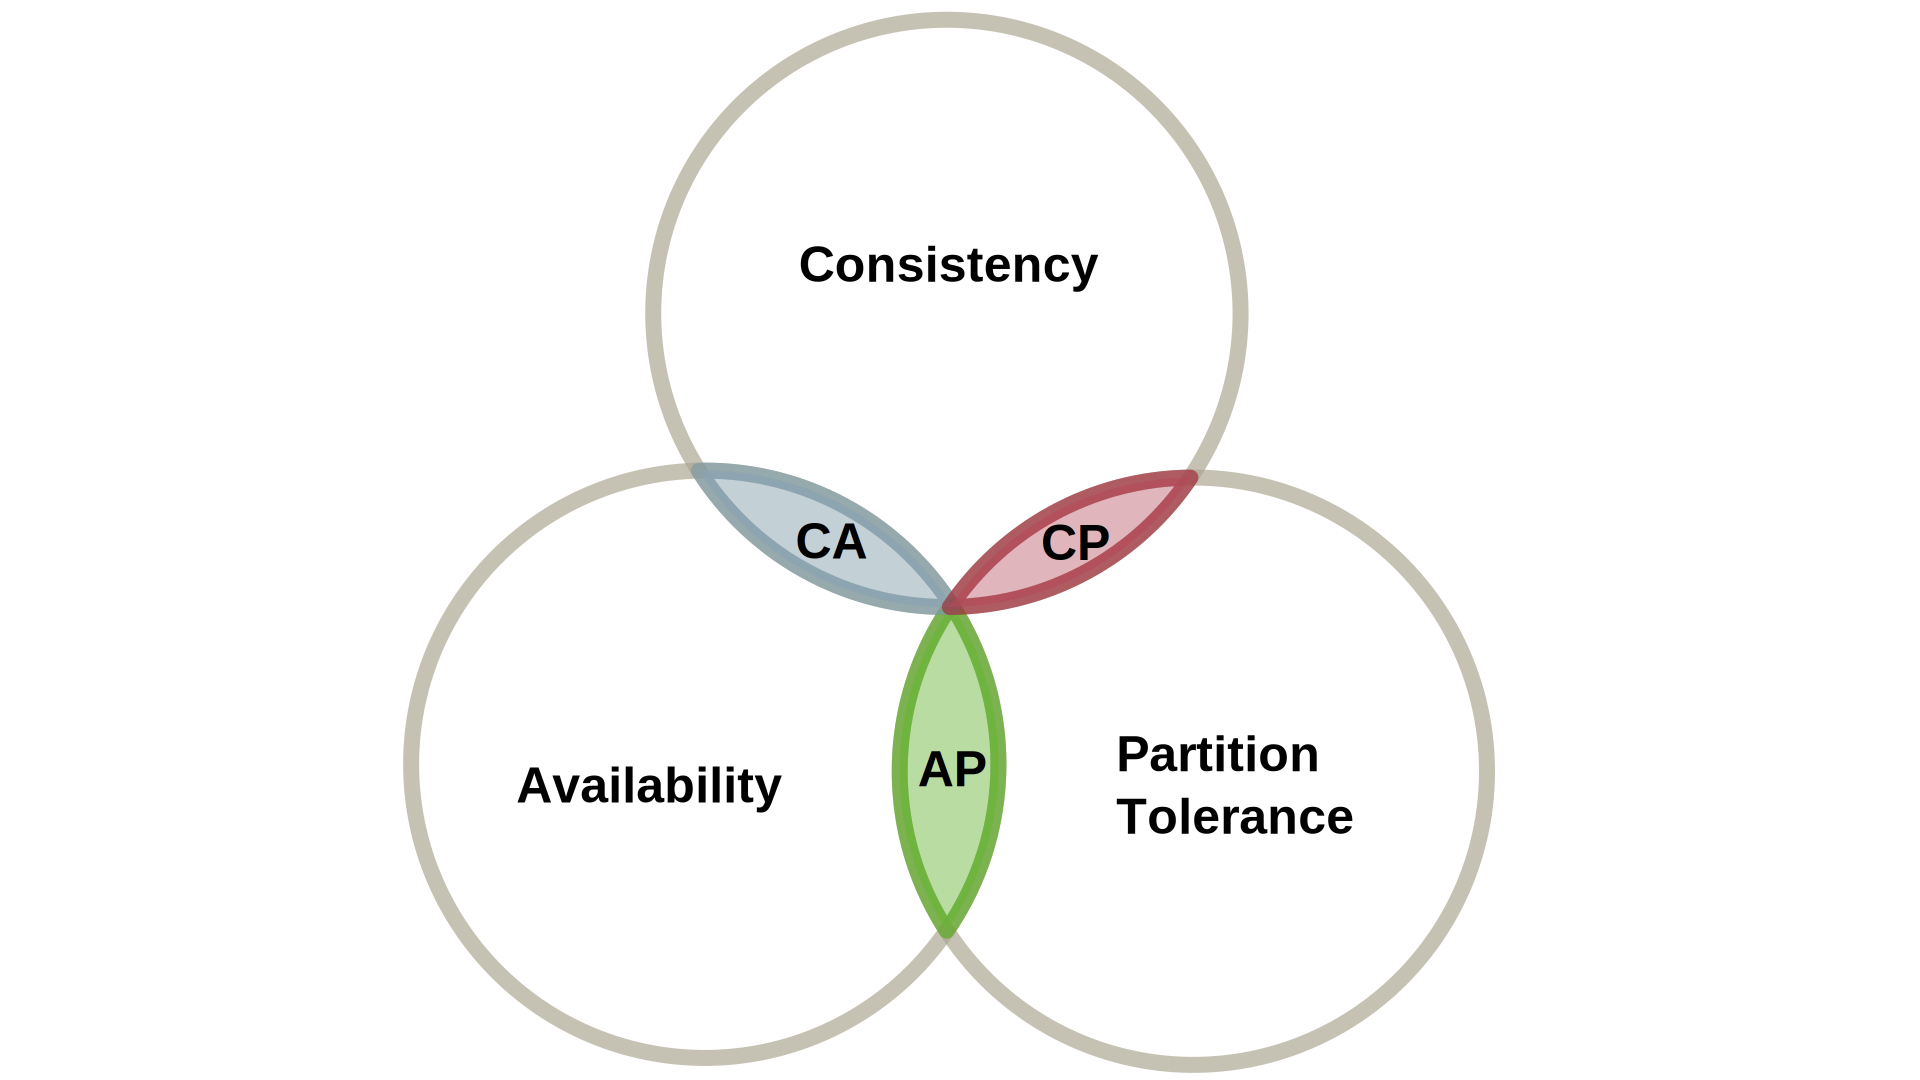
\includegraphics[width=0.8\textwidth]{images/cap.pdf}
	\caption{Übersicht der Project Helin Architektur }
	\label{fig:architecture-overview}
\end{figure}

\begin{itemize}
	\item{\textbf{Consistency:} Guarantees that a read will receive the most recent data or an error.}
	\item{\textbf{Availability:} Every request will get a response, although no guarantee on correctness of the data. }
	\item{\textbf{Partition Tolerance:} The system can operate although parts of it are unavailable due to network or hardware failure.}
	
\end{itemize}


\begin{tabular}{lll}


\end{tabular}

\begin{figure}[H]
	\centering
	\includegraphics[scale=1]{images/DBMS_overview.png}
	\caption{Übersicht der Project Helin Architektur }
	\label{fig:architecture-overview}
\end{figure}


\begin{figure}[H]
	\centering
%	\includegraphics[width=1\textwidth]{images/DSMS_overview.png}
	\caption{Übersicht der Project Helin Architektur }
	\label{fig:architecture-overview}
\end{figure}
